\documentclass[12pt]{beamer}
% \usetheme{umbc4}
\usetheme{moloch}

\usepackage{amsmath,amscd}
\usepackage{fontspec}
\usepackage{unicode-math}
\usepackage{pifont}
\usepackage{xcolor}
\usepackage[dvipsnames]{xcolor}
\usepackage{listings}
\usepackage{minted}
\usepackage{tikz}

\setmonofont{DejaVu Sans Mono}

% Set the title bar to black background with white text
\setbeamercolor{frametitle}{bg=black, fg=white}

% Ensure other structural elements (bullets, etc.) are visible
\setbeamercolor{structure}{fg=white}

\setmainfont{Libertinus Serif}
\setsansfont{Libertinus Sans}
\setmathfont{STIX Two Math}

% Define colors for syntax highlighting
\definecolor{codegreen}{rgb}{0,0.6,0}
\definecolor{codegray}{rgb}{0.5,0.5,0.5}
\definecolor{codecoffee}{rgb}{0.75,0.6,0.3}
\definecolor{question}{rgb}{1.0,0.75,0.1}
\definecolor{lightblue}{rgb}{0.55,0.75,0.9}
\definecolor{yellow}{rgb}{1.0, 1.0, 0.0}
\definecolor{codecomment}{rgb}{0.97, 0.74, 0.4}
\definecolor{codepy}{rgb}{0.9, 0.85, 0.85} %{#F8BC65}
\definecolor{funcColor}{rgb}{0.47, 0.6, 0.8}
\definecolor{midgray}{rgb}{0.4, 0.4, 0.3}
\definecolor{indexwhite}{rgb}{0.9, 0.9, 0.9}

\setbeamercolor{background canvas}{bg=black}
\setbeamercolor{normal text}{fg=white}

\newcommand{\FrameTitle}[2]{\frametitle{#1 \hfill \small\textnormal{\textcolor{midgray}{#2}}}}
\newcommand{\snl}{\vspace*{6pt}\\}
\newcommand{\nl}{\vspace*{1em}\\}
\newcommand{\vsp}{\vspace*{1em}}


\lstdefinestyle{mypystyle}{
    commentstyle=\color{codecomment},
    keywordstyle=\color{lightblue},
    numberstyle=\scriptsize\color{codegray},
    stringstyle=\color{codecoffee},
    basicstyle=\ttfamily\scriptsize\color{codepy},
    breakatwhitespace=false,
    breaklines=true,
    lineskip=2pt,  % introduces a small gap between lines for better readability
    % captionpos=b,
    keepspaces=true,
    numbers=left,
    numbersep=5pt,
    firstnumber=1,  % Forces reset to 1 for EVERY listing
    showspaces=false,
    showstringspaces=false,
    showtabs=false,
    tabsize=2,
    language=Python,
    backgroundcolor=\color{black},
    emph=[2]{__init__, calculate},
    emphstyle=[2]\color{funcColor},
}
\lstset{style=mypystyle}

\setminted{
    style=mymintstyle,    % High contrast light theme
    fontsize=\ttfamily\scriptsize, % Slightly smaller to fit more code, but still readable
    breaklines,           % Prevents code from running off the slide
    baselinestretch=1.2,  % Increases line height by 25%
    framesep=0mm,         % Padding inside the frame
    % frame=lines,        % Optional: adds top/bottom lines for definition
    bgcolor=black,
    mathescape,
    breaklines=true,
    tabsize=2,
    xleftmargin=1mm,
    linenos,              % Enable line numbers
    %linenosstyle=bold,   % Optional: make them bold for visibility
    numbersep=2mm,        % Space between number and code
}

% Define your custom line number style
\renewcommand{\theFancyVerbLine}{%
  \sffamily\textcolor{gray}{\scriptsize\arabic{FancyVerbLine}}
}

\usemintedstyle{mymint}

\begin{document}
\title{\center{Applied Linear Algebra \\\vsp NumPy and PyTorch \\}}

\author{\center{Devi Prasad M \\ Manipal School of Information Sciences \\ Manipal \\}}
\date{\center{Monday, 3 August 2026}}
\maketitle

\begin{frame}[fragile]\FrameTitle{Array Basics}{NumPy}
    Try the following in a Python shell\nl

    \begin{lstlisting}{python}
        import numpy as np

        a = np.array([1, 2, 3])

        assert(a.dtype == np.int64)

        # what is the shape of 'a'?
        assert(a.shape == ?)
    \end{lstlisting}
\end{frame}

\begin{frame}[fragile]\FrameTitle{Array Shape}{NumPy}
\begin{lstlisting}{python}
    import numpy as np

    a = np.array([1, 2, 3])
    assert(a.shape == (3,))

    assert(a.shape != (3)) # why?
    assert(a.shape != 3) # why so?

    ## what's the type of a.shape?
    assert(isinstance(a.shape, ?))
\end{lstlisting}
\end{frame}


\begin{frame}[fragile]\FrameTitle{Array of Zeroes}{NumPy}
\begin{lstlisting}{python}
    import numpy as np

    a = np.zeros(4)
    assert a == [0, 0, 0, 0] # what's up with is?

    # 'array_equal'
    assert np.array_equal(a, [0, 0, 0, 0])

    # explain this!
    assert (a == np.array([0, 0, 0, 0])).all()

    # what's the type of a.shape?
    assert(isinstance(a.shape, ?))
\end{lstlisting}
\end{frame}


\begin{frame}[fragile]\FrameTitle{1-Dimensional ndarray}{NumPy}
\begin{lstlisting}{python}
    import numpy as np

    a = np.array([0.12, 0.45, 0.78, 1.34, 2.91])
    assert(a.shape == (5,))
    assert(a.ndim == 1)
    assert(a.size == 5)
\end{lstlisting}

\centering\hspace*{6mm}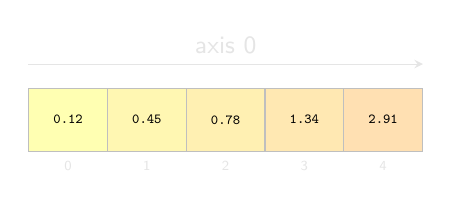
\begin{tikzpicture}
    \def\arraydata{0.12, 0.45, 0.78, 1.34, 2.91}
    \foreach \val [count=\i from 0, evaluate=\i as \gradient using int(\i*20)] in \arraydata {
        \node(node-\i)[
            draw=gray!50,
            thin,
            text=black,
            fill=orange!\gradient!yellow!30,
            minimum height=0.8cm,
            minimum width=1cm,
            anchor=west,
            label={[text=indexwhite, font=\tiny\sffamily]below:\i}
        ]
        at (\i*1cm, 0) {\tiny\texttt{\val}};
    }

    %\draw[->, thin, >=stealth, indexwhite] (node-4.east) -- ++(1.1, 0)
    %    node[right, font=\small\sffamily] {axis 0};

    \draw[->, thin, >=stealth, indexwhite] ([yshift=0.3cm]node-0.north west) -- ([yshift=0.3cm]node-4.north east)
        node[midway, above, text=indexwhite, font=\small\sffamily] {axis 0};


\end{tikzpicture}
\end{frame}

\begin{frame}[fragile]\FrameTitle{2-Dimensional ndarray}{NumPy}
\begin{lstlisting}[language=Python]
    # A 3x5 2D ndarray/tensor
    a = np.array([
        [0.12, 0.45, 0.78, 1.34, 2.91],
        [0.23, 0.56, 0.89, 1.45, 3.02],
        [0.34, 0.67, 0.90, 1.56, 3.13],
    ])
    assert(a.shape == (3, 5))
    assert(a.ndim == 2)
\end{lstlisting}

\vspace{0.3cm}

\centering
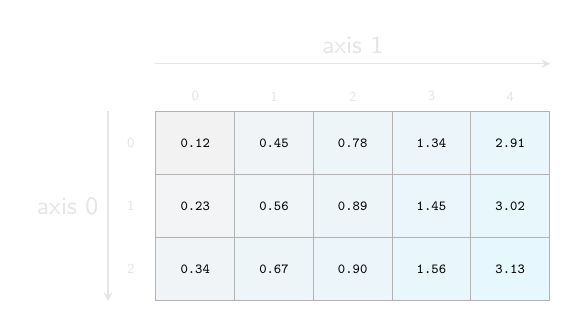
\begin{tikzpicture}
    % Define the 2D data matrix elements
    \def\rowZero{0.12, 0.45, 0.78, 1.34, 2.91}
    \def\rowOne{0.23, 0.56, 0.89, 1.45, 3.02}
    \def\rowTwo{0.34, 0.67, 0.90, 1.56, 3.13}

    \foreach \r in {0, 1, 2} {
        \ifnum\r=0 \let\cols=\rowZero \fi
        \ifnum\r=1 \let\cols=\rowOne \fi
        \ifnum\r=2 \let\cols=\rowTwo \fi

        \foreach \val [count=\c from 0, evaluate=\c as \gradient using int(\c*20 + \r*10)] in \cols {

            % Draw cell (black text on bright gradient fills is highly readable)
            \node(cell-\r-\c)[
                draw=gray!60,         % Made cell borders slightly brighter gray
                thin,
                text=black,
                fill=cyan!\gradient!gray!10,  % Adjusted gradient for better contrast
                minimum height=0.8cm,
                minimum width=1.0cm,
                anchor=north west
            ] at (\c*1.0cm, -\r*0.8cm) {\tiny\texttt{\val}};

            % Column Indices (axis 1) - rendered in bright indexwhite
            \ifnum\r=0
                \node[text=indexwhite, font=\tiny\sffamily, above] at (cell-\r-\c.north) {\c};
            \fi
        }

        % Row Indices (axis 0) - rendered in bright indexwhite
        \node[text=indexwhite, font=\tiny\sffamily, left=4pt] at (cell-\r-0.west) {\r};
    }

    % Axis 1 (Columns): Horizontal arrow running left-to-right above the entire matrix
    \draw[->, thin, >=stealth, indexwhite] ([yshift=0.6cm]cell-0-0.north west) -- ([yshift=0.6cm]cell-0-4.north east)
        node[midway, above, text=indexwhite, font=\small\sffamily] {axis 1};

    % Axis 0 (Rows): A vertical arrow running down the left side of the entire matrix
    \draw[->, thin, >=stealth, indexwhite] ([xshift=-0.6cm]cell-0-0.north west) -- ([xshift=-0.6cm]cell-2-0.south west)
    node[midway, left, text=indexwhite, font=\small\sffamily] {axis 0};

\end{tikzpicture}
\end{frame}


\begin{frame}[fragile]\FrameTitle{3-Dimensional ndarray}{NumPy}
\begin{lstlisting}[language=Python]
    import numpy as np

    # A 3x3x4 3D tensor: shape (planes, rows, cols)
    a = np.random.rand(3, 3, 4)
    assert(a.shape == (3, 3, 4))
    assert(a.ndim == 3)
\end{lstlisting}

\vspace{0.1cm}

\centering
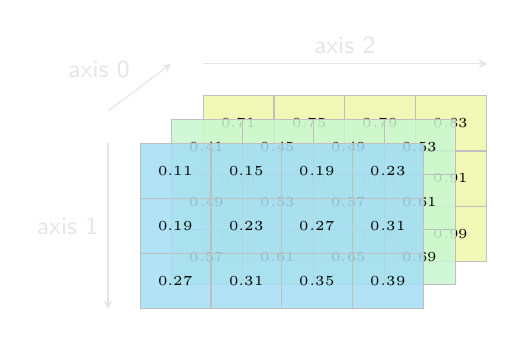
\begin{tikzpicture}[
    % Set up a 3D projection style
    cell/.style={
        draw=gray!50,
        thin,
        text=black,
        minimum height=0.7cm,
        minimum width=0.9cm,
        anchor=north west,
        fill opacity=0.85, % Semi-transparent so you can see back layers!
        text opacity=1.0
    }
]
    % Loop through Depth (d), Rows (r), and Columns (c)
    % We evaluate \colormix: 0 (front/blue) -> 45 (middle/greenish-blue) -> 90 (back/yellow)
    \foreach \d [evaluate=\d as \colormix using int(\d*45)] in {2, 1, 0} {
        \foreach \r in {0, 1, 2} {
            \foreach \c in {0, 1, 2, 3} {

                % Standard numeric gradient for cell value variation within the layer
                \pgfmathsetmacro{\cellval}{0.11 + \d*0.3 + \r*0.08 + \c*0.04}

                % We blend yellow and cyan based on depth, then apply a matte gray finish
                \node(cell-\d-\r-\c)[
                    cell,
                    fill=yellow!\colormix!cyan!85!gray!40
                ] at (\c*0.9cm + \d*0.4cm, -\r*0.7cm + \d*0.3cm) {
                    \tiny\texttt{\pgfmathprintnumber[fixed, precision=2]{\cellval}}
                };
            }
        }
    }

    % --- 3D AXIS INDICATORS (Sparsely labeled for maximum clarity) ---

    % Axis 2 (Columns): Horizontal arrow pointing right along the front-most layer
    \draw[->, thin, >=stealth, indexwhite] ([yshift=0.4cm]cell-2-0-0.north west) -- ([yshift=0.4cm]cell-2-0-3.north east)
        node[midway, above, text=indexwhite, font=\small\sffamily] {axis 2};

    % Axis 1 (Rows): Vertical arrow pointing down along the front-most layer
    \draw[->, thin, >=stealth, indexwhite] ([xshift=-0.4cm]cell-0-0-0.north west) -- ([xshift=-0.4cm]cell-0-2-0.south west)
        node[midway, left, text=indexwhite, font=\small\sffamily] {axis 1};

    % Axis 0 (Depth/Planes): Projected arrow pointing from front to back
    \draw[->, thin, >=stealth, indexwhite] ([xshift=-0.4cm, yshift=0.4cm]cell-0-0-0.north west) -- ([xshift=-0.4cm, yshift=0.4cm]cell-2-0-0.north west)
        node[midway, above left, text=indexwhite, font=\small\sffamily] {axis 0};
\end{tikzpicture}
\end{frame}

\end{document}
